% !TeX root = ../main.tex
% Add the above to each chapter to make compiling the PDF easier in some editors.

\chapter{Background}\label{chapter:background} % Anshul 4 sayfa yazmış

\section{Cloud Computing Landscape} % Cloud usage scenarios
\subsection{Usage Scenarios}
Cloud computing is becoming increasingly popular as on-demand provisioning capabilities and support for various use cases are growing. Cloud computing is currently being used in many different aspects of our lives. \cite{cloud-use-cases} Some of those aspects include file storage like OneDrive, database as a service systems like Amazon SimpleDB, entertainment services such as Netflix, multiplayer online games like Dota 2. Businesses are also using cloud computing for instant messaging between departments through applications like Slack or storing customer data in customer relationship management services provided by companies such as SAP or Salesforce. Many businesses also offload their computing requirements to cloud for data mining or for project management, as the Pay-per-use model of cloud is very beneficial for companies because they don't need to maintain a cluster of computers in premise. Cloud computing is also being used to host massive websites such as Facebook.com or Amazon.com.
\subsection{Virtualization}
The different use cases explained above are only possible because cloud computing provides abstraction by virtualisation. Real hardware in data centers can be abstracted and be broken to smaller units and be distributed to customers as virtual machines. That way every customer can have their own personal computer running on the cloud and their system is fully isolated from other customers. While virtual machines were the defacto unit in cloud computing for many years, now there is a new technology called \textit{containerisation}. Contaniers allow applications to be packed with their dependencies, and those application can run on the same host OS on top of a container engine. That allows for better utilized servers and less dependency from the underlying hardware. It comes with a cost though. Containers add another layer of abstraction on the stack thus they have a delay. 

This abstraction is possible with hypervisor technologies such as Xen. Controlled by software APIs, hypervisors boot self-contained computers on demand, and can run applications as if they were running on physical hosts. This is called \textit{server consolidation} and it has been a great way to reduce under-utilized hardware. 

\iffalse
\begin{figure}[htpb]
  \centering
  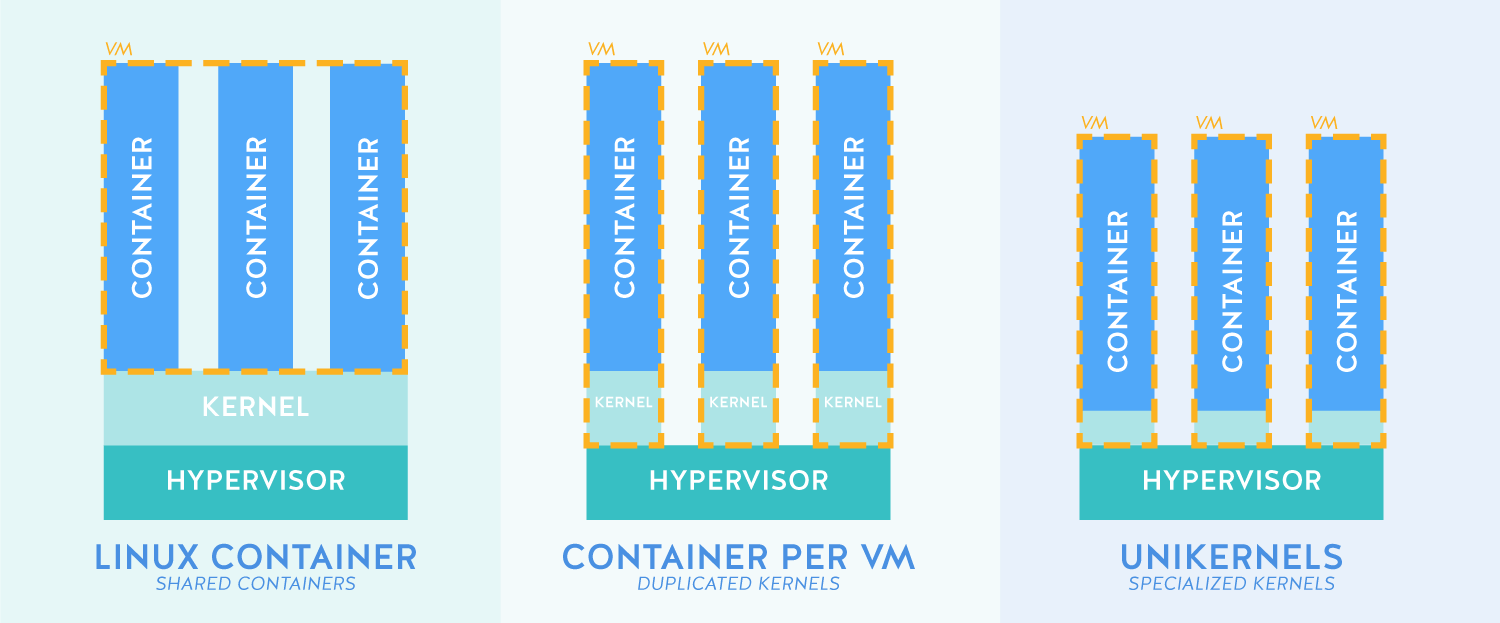
\includegraphics[width=0.4\textwidth]{figures/Linux-containers-vms-unikernels.png}
  \caption{Different virtualization techniques: https://nordicapis.com/introduction-to-unikernels/} \label{fig:virt}
\end{figure}
\fi
\section{Unikernels}
Unikernels \cite{library-operating-system} \cite{madhavapeddy2014unikernels} are specialised machine images compiled from high-level languages. Those machine images can run directly on the hypervisor or on the bare metal. First examples of unikernels can be seen from the late 1990's from the projects like Exodus\cite{exokernel} and Nemesis \cite{nemesis}. In a unikernel project, the developer selects libraries from a repository where the OS functionalities are implemented. In most cases, these libraries are also implemented in the high-level language that the project is implemented. Once the required libraries for the project are selected, whole codebase is compiled with configuration code for the target system. The resulting artifact has the modular stack architecture similar to figure \ref{fig:unikernel-arch} and is a single OS image. This OS image can than be distributed similar to conventional OS images and be booted directly by hypervisor or directly on the hardware. They can be uploaded to cloud systems like OpenStack \cite{openstack} to be booted at will or can be distributed to smaller devices, which is the purpose of this project.

\begin{figure}[htpb]
  \
  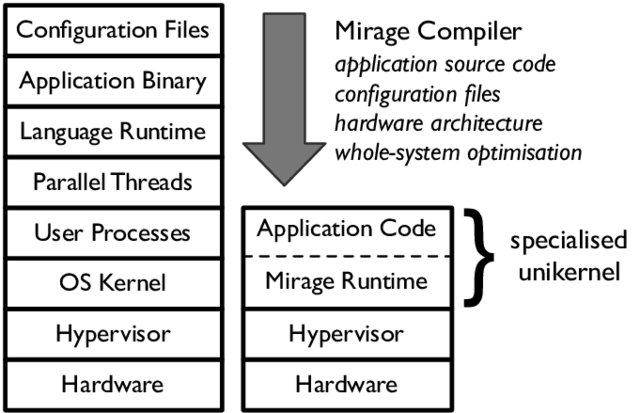
\includegraphics[height=0.3\textwidth]{figures/Contrasting-software-layers-in-existing-VM-appliances-vs-unikernels-standalone-kernel_W640.jpg}
  \caption{ Contrasting software layers in existing VM appliances vs. unikernel’s standalone kernel compilation approach. \cite{library-operating-system}} \label{fig:unikernel-arch}
\end{figure}

Unikernels are currently not production ready. \cite{unfit-for-production} They lack the proper tooling around them and they don't have a "killer-app" for now. Nevertheless there is a growing interest around them with startups trying to bring the technology to general usage. One of those start-ups is Unikernel Systems, based in Cambridge, UK. Unikernel Systems was acquired by Docker in 2016 \cite{docker-acquisiton}. The company consists mostly of developers from the Xen Project. Unikernel technology is more low-level than what Docker provides with it's containers and they stated that they want to use low-level programming expertise of the unikernel team to enchance the power of Docker. All these connections between those three components, namely Docker, Unikernel System and ex-Xen developers show us the big picture of cloud techology.

The advantages and drawbacks of using unikernels is explained more in the implementation part of the this thesis with encountered problems and solutions.

\section{Orchestration}
IT adoption of the containers is still low but it's growing every year. A survey made by Diamante states that "in 2018 just 17 percent said that IT operations teams were driving container adoption; a year later that number has jumped to more than 35 percent" \cite{diamante}. They also state that the reason for this big shift is the advances in orchestration technology. Currently the most popular orchestration technology is Kubernetes , an open source project, initiated by Google. Kubernetes connects multiple machines together and serves their resources through a single interface for container deployment. It takes the responsibility of running containers from developers and puts them on automation algorithm. It's treating containers as short lived entities and deploys them again if a container fails or if a better resource utilization oppurtunity is available.

Kubernetes also has a communication interface between machines for containers to talk with each other and with outside services. This communication is possible with a kubernetes daemon called kubelet running on every machine connected to the cluster. This intercluster networking is realised by an internal DNS and load balancers. This networking can be extended by the user with a resource called "Service". With that, different deployments can talk to each other through kubernetes without requiring an explicit IP address. All low level communication is handled by the kubernetes stack. 

Kubernetes' internal load balancer is also useful for scaling. Kubernetes has a scaling functionality for busy containers. If a deployment is taking to much request, K8S creates replicas of the container, possibly on different machines, thus divides the incoming workload. This is called vertical scaling as if no custom scaling algorithm is given, handled completely by the cluster. Many cloud providers provide Kubernetes clusters as products, e.g. Google Kubernetes Engine or Amazon Elastic Kubernetes Engine, and if desired, they also increase the number of machines in the cluster if there is no more space left to deploy more replicas.

It's popularity comes from the fact it was being used by Google for their internal systems and it's ability to abstract hardware from the deployed software. It also aligns well with the microservices paradigm. While bigger applications are being divided to smaller units, Kubernetes clusters can support up to 150,000 pods \cite{kubernetes-load}, kubernetes' smallest unit. It is also very customizable and there are many products on top of it to deal with the complexity. Some projects that are very popular around the Kubernetes ecosystem , e.g. Istio \cite{istio} for service meshing, which allows better customisation of inter-cluster communication, Helm \cite{helm} for package manager of kubernetes applications or Envoy \cite{envoy} as a service proxy.

While Kubernetes is the most dominant orchestration technology on the market right now, there are alternative technologies too. Some of those technologies are Nomad, Apache Mesos and OpenShift.

\newpage
\section{Managing IoT}
Cheaper and faster computational resources allowed developers to put small computers on everyday devices. Other than smartphones , we now have smart refrigerators, smart watches , smart street lights and smart cities. All of this is not only possible with improvements in the computation technology but also with improvements within communication. There are newer protocols for bandwidth and battery friendly communication between restricted devices. This ecosystem of connected devices is called Internet of Things. There is expected to be "20 billion to 35 billion"\cite{unikernels-improve} connected devices in 2020. While that numbers can be a great producer of data and increases the usage of cloud for those scenarios, it brings it's own problems, namely security and complexity.

The repeating problems of IoT is security and complexity. The field is a new field in terms of developer activity and there are no established standards on how to make it more secure. While enterprise security problem is pretty much solved with a centralised firewall approach but that only works if the servers are on-premise and in a physically isolated places. IoT, by nature, is out in the public and highly distributed. A corporate based solution does not work for IoT, because a bad actor has physical access to the device and can tinker with it. They can attack it through hardware or by modifying the environment where the device is running. The resource constraint of IoT devices also make it hard to embed encryption algorithms in them to protect data locally. This problem ask for a solution that is yet to be implemented.

The complexity problem of IoT comes from the number of devices out there in the public. It is impossible to manage deployed devices manually, where they might require updates on the software, redefined tasks... There are technologies to enable local, self organizing IoT clusters like Zigbee or 6LoWPAN but they don't solve the problem of hiearchy. While does tehnologies allow close proximity devices talk to each other, IoT devices still require a central authority to send data to and to tell them what to do.

%Todo: those techs are called mesh networks
%TODO: maybe add cites to technologies
